% ============================================================
% SLIDE BÁO CÁO ĐỒ ÁN TỐT NGHIỆP
% Biên dịch bằng: xelatex (bắt buộc, cần font Times New Roman)
% ============================================================
\documentclass[aspectratio=43,10pt]{beamer}

% --- Theme ---
\usetheme{Madrid}
\usecolortheme{default}

% --- Encoding & Font ---
\usepackage{fontspec}
\usepackage[vietnamese]{babel}
\setmainfont{Times New Roman}

% --- Graphics & Color ---
\usepackage{graphicx}
\graphicspath{{hinh_latex/}}
\usepackage{tikz}
\usetikzlibrary{shapes.geometric, arrows.meta, positioning, fit, backgrounds, calc}

% --- Tables ---
\usepackage{booktabs}
\usepackage{array}

% --- TikZ styles ---
\tikzstyle{block} = [rectangle, rounded corners, minimum width=2.5cm, minimum height=1cm, align=center, inner sep=2mm, draw=black, fill=blue!8, font=\small]
\tikzstyle{decision} = [diamond, aspect=2.5, minimum width=2cm, align=center, inner sep=1mm, draw=black, fill=yellow!15, font=\small]
\tikzstyle{arrow} = [thick, ->, >=Stealth]
\tikzstyle{darrow} = [thick, <->, >=Stealth]
\tikzstyle{process} = [rectangle, minimum width=2cm, minimum height=0.8cm, align=center, inner sep=2mm, draw=black, fill=green!8, font=\small]
\tikzstyle{reject} = [rectangle, rounded corners, minimum width=2cm, minimum height=0.8cm, align=center, inner sep=2mm, draw=red!70, fill=red!8, font=\small]
\tikzstyle{accept} = [rectangle, rounded corners, minimum width=2cm, minimum height=0.8cm, align=center, inner sep=2mm, draw=green!70!black, fill=green!12, font=\small]

% --- Title Info ---
\title[Hệ thống bãi đỗ xe tự động]{BÁO CÁO ĐỒ ÁN TỐT NGHIỆP\\HỆ THỐNG BÃI ĐỖ XE TỰ ĐỘNG ỨNG DỤNG NHẬN DIỆN BIỂN SỐ}
\author[Sinh viên thực hiện]{Sinh viên thực hiện: ...\\Giảng viên hướng dẫn: ...}
\institute[KHOA CNTT]{KHOA CÔNG NGHỆ THÔNG TIN\\TRƯỜNG ĐẠI HỌC ...}
\date{Năm 2026}

\begin{document}

\begin{frame}
    \titlepage
\end{frame}

\begin{frame}{Nội dung báo cáo}
    \tableofcontents
\end{frame}

% --- Phần 1: Giới thiệu ---
\section{Giới thiệu chung}
\begin{frame}{1. Đặt vấn đề}
    \begin{itemize}
        \item \textbf{Thực trạng:} Các bãi đỗ xe truyền thống quản lý thủ công (ghi vé giấy, quẹt thẻ) tốn nhân lực, dễ xảy ra sai sót, ùn tắc vào giờ cao điểm.
        \item \textbf{Giải pháp:} Ứng dụng AI để nhận diện biển số xe tự động, kết hợp với hệ thống phần cứng điều khiển barrier.
        \item \textbf{Mục tiêu:}
        \begin{itemize}
            \item Xây dựng mô hình AI nhận diện biển số với độ chính xác cao.
            \item Xây dựng phần mềm quản lý trên máy tính (Giao diện UI, CSDL).
            \item Tích hợp phần cứng Arduino và cảm biến để tự động đóng/mở cổng.
        \end{itemize}
    \end{itemize}
\end{frame}

% --- Phần 2: Cơ sở lý thuyết ---
\section{Cơ sở lý thuyết}
\begin{frame}{2. Cơ sở lý thuyết: Mô hình YOLOv8}
    \begin{itemize}
        \item \textbf{YOLO (You Only Look Once):} Là họ mô hình phát hiện đối tượng (Object Detection) thời gian thực.
        \item \textbf{YOLOv8:} Phiên bản mới nhất với kiến trúc không cần điểm neo (anchor-free), tối ưu tốc độ và độ chính xác.
        \item \textbf{Vai trò:} Dùng để dò tìm và khoanh vùng (bounding box) vị trí của biển số xe trên ảnh camera đầu vào.
    \end{itemize}
\end{frame}

\begin{frame}{2. Cơ sở lý thuyết: PaddleOCR}
    \begin{itemize}
        \item \textbf{PaddleOCR:} Là bộ công cụ nhận dạng ký tự quang học (OCR) mã nguồn mở.
        \item \textbf{Ưu điểm:} Hỗ trợ đa ngôn ngữ, rất nhẹ, mô hình được tối ưu hóa cho thiết bị có tài nguyên thấp.
        \item \textbf{Vai trò:} Đọc các ký tự (số và chữ) từ ảnh vùng biển số đã được YOLOv8 cắt ra.
    \end{itemize}
\end{frame}

% --- Phần 3: Thiết kế hệ thống ---
\section{Thiết kế hệ thống}
\begin{frame}{3. Sơ đồ khối tổng thể}
    \begin{center}
    \resizebox{0.9\textwidth}{!}{%
    \begin{tikzpicture}[node distance=1.2cm and 2cm, every node/.style={font=\small}]
        \node[block, fill=cyan!15] (cam) {Camera\\(Thu nhận ảnh)};
        \node[block, fill=orange!15, right=1.5cm of cam] (ai) {Khối xử lý AI\\(YOLOv8 + OCR)};
        \node[block, fill=green!15, right=1.5cm of ai] (db) {Cơ sở dữ liệu\\(SQLite)};
        \node[block, fill=yellow!15, below=1.5cm of ai] (ui) {Giao diện\\(Tkinter)};
        \node[block, fill=purple!15, below=1.5cm of cam] (hw) {Phần cứng\\(Arduino + Servo)};
        
        \draw[arrow] (cam) -- (ai);
        \draw[darrow] (ai) -- (db);
        \draw[darrow] (ai) -- (ui);
        \draw[arrow] (ui) -- (hw);
        \draw[arrow] (hw) -- (ui);
    \end{tikzpicture}
    }
    \end{center}
\end{frame}

\begin{frame}{3. Pipeline nhận diện biển số}
    \begin{center}
    \resizebox{1\textwidth}{!}{%
    \begin{tikzpicture}[node distance=1cm and 1.5cm, every node/.style={font=\small}]
      % Hàng 1 (trái sang phải)
      \node[block, fill=cyan!15] (cam) {Ảnh camera\\(BGR frame)};
      \node[block, fill=orange!15, right=of cam] (yolo) {YOLOv8\\Phát hiện vùng};
      \node[block, fill=yellow!12, right=of yolo] (crop) {Crop\\vùng biển số};
      
      % Hàng 2 (chia 3 nhánh)
      \node[process, below=of crop] (clahe) {CLAHE};
      \node[process, left=of clahe] (goc) {Ảnh gốc};
      \node[process, right=of clahe] (otsu) {Otsu};
      
      % Hàng 3 (phải sang trái)
      \node[block, fill=purple!12, below=of clahe] (ocr) {PaddleOCR};
      \node[block, fill=green!12, left=of ocr] (hxl) {Hậu xử lý\\+ Chấm điểm};
      \node[accept, left=of hxl] (kq) {Biển số\\cuối cùng};
      
      % Mũi tên
      \draw[arrow] (cam) -- (yolo);
      \draw[arrow] (yolo) -- (crop);
      
      \draw[arrow] (crop) -- (goc);
      \draw[arrow] (crop) -- (clahe);
      \draw[arrow] (crop) -- (otsu);
      
      \draw[arrow] (goc) -- (ocr);
      \draw[arrow] (clahe) -- (ocr);
      \draw[arrow] (otsu) -- (ocr);
      
      \draw[arrow] (ocr) -- (hxl);
      \draw[arrow] (hxl) -- (kq);
    \end{tikzpicture}
    }
    \end{center}
\end{frame}

\begin{frame}{3. Sơ đồ phần cứng}
    \begin{center}
    \resizebox{0.7\textwidth}{!}{%
    \begin{tikzpicture}[node distance=1.2cm, every node/.style={font=\small}]
      \node[block, fill=gray!20, minimum width=4cm] (pc) {Máy tính\\Python Software};
      \node[block, fill=blue!15, minimum width=4cm, below=1.5cm of pc] (ard) {Arduino Uno};
      
      \node[block, fill=green!15, below left=2cm and 1cm of ard] (sv1) {Servo cổng VÀO\\(D9 - PWM)};
      \node[block, fill=green!15, below right=2cm and 1cm of ard] (sv2) {Servo cổng RA\\(D10 - PWM)};
      \node[block, fill=yellow!15, left=2cm of ard] (cb1) {LM393 cổng VÀO\\(D2 - Digital)};
      \node[block, fill=yellow!15, right=2cm of ard] (cb2) {LM393 cổng RA\\(D3 - Digital)};
      
      \draw[darrow] (pc) -- node[right, font=\scriptsize, align=center]{USB Serial 9600 baud} (ard);
      \draw[arrow] (ard) -- node[left, font=\scriptsize]{PWM} (sv1);
      \draw[arrow] (ard) -- node[right, font=\scriptsize]{PWM} (sv2);
      \draw[arrow] (cb1) -- node[above, font=\scriptsize]{DO} (ard);
      \draw[arrow] (cb2) -- node[above, font=\scriptsize]{DO} (ard);
    \end{tikzpicture}
    }
    \end{center}
\end{frame}

% --- Phần 4: Kết quả ---
\section{Kết quả đạt được}
\begin{frame}{4. Kết quả huấn luyện YOLOv8}
    \begin{itemize}
        \item Huấn luyện trên bộ dữ liệu \textbf{16,112 ảnh} (Roboflow).
        \item Số epoch: \textbf{50}.
    \end{itemize}
    \begin{figure}
        \centering
        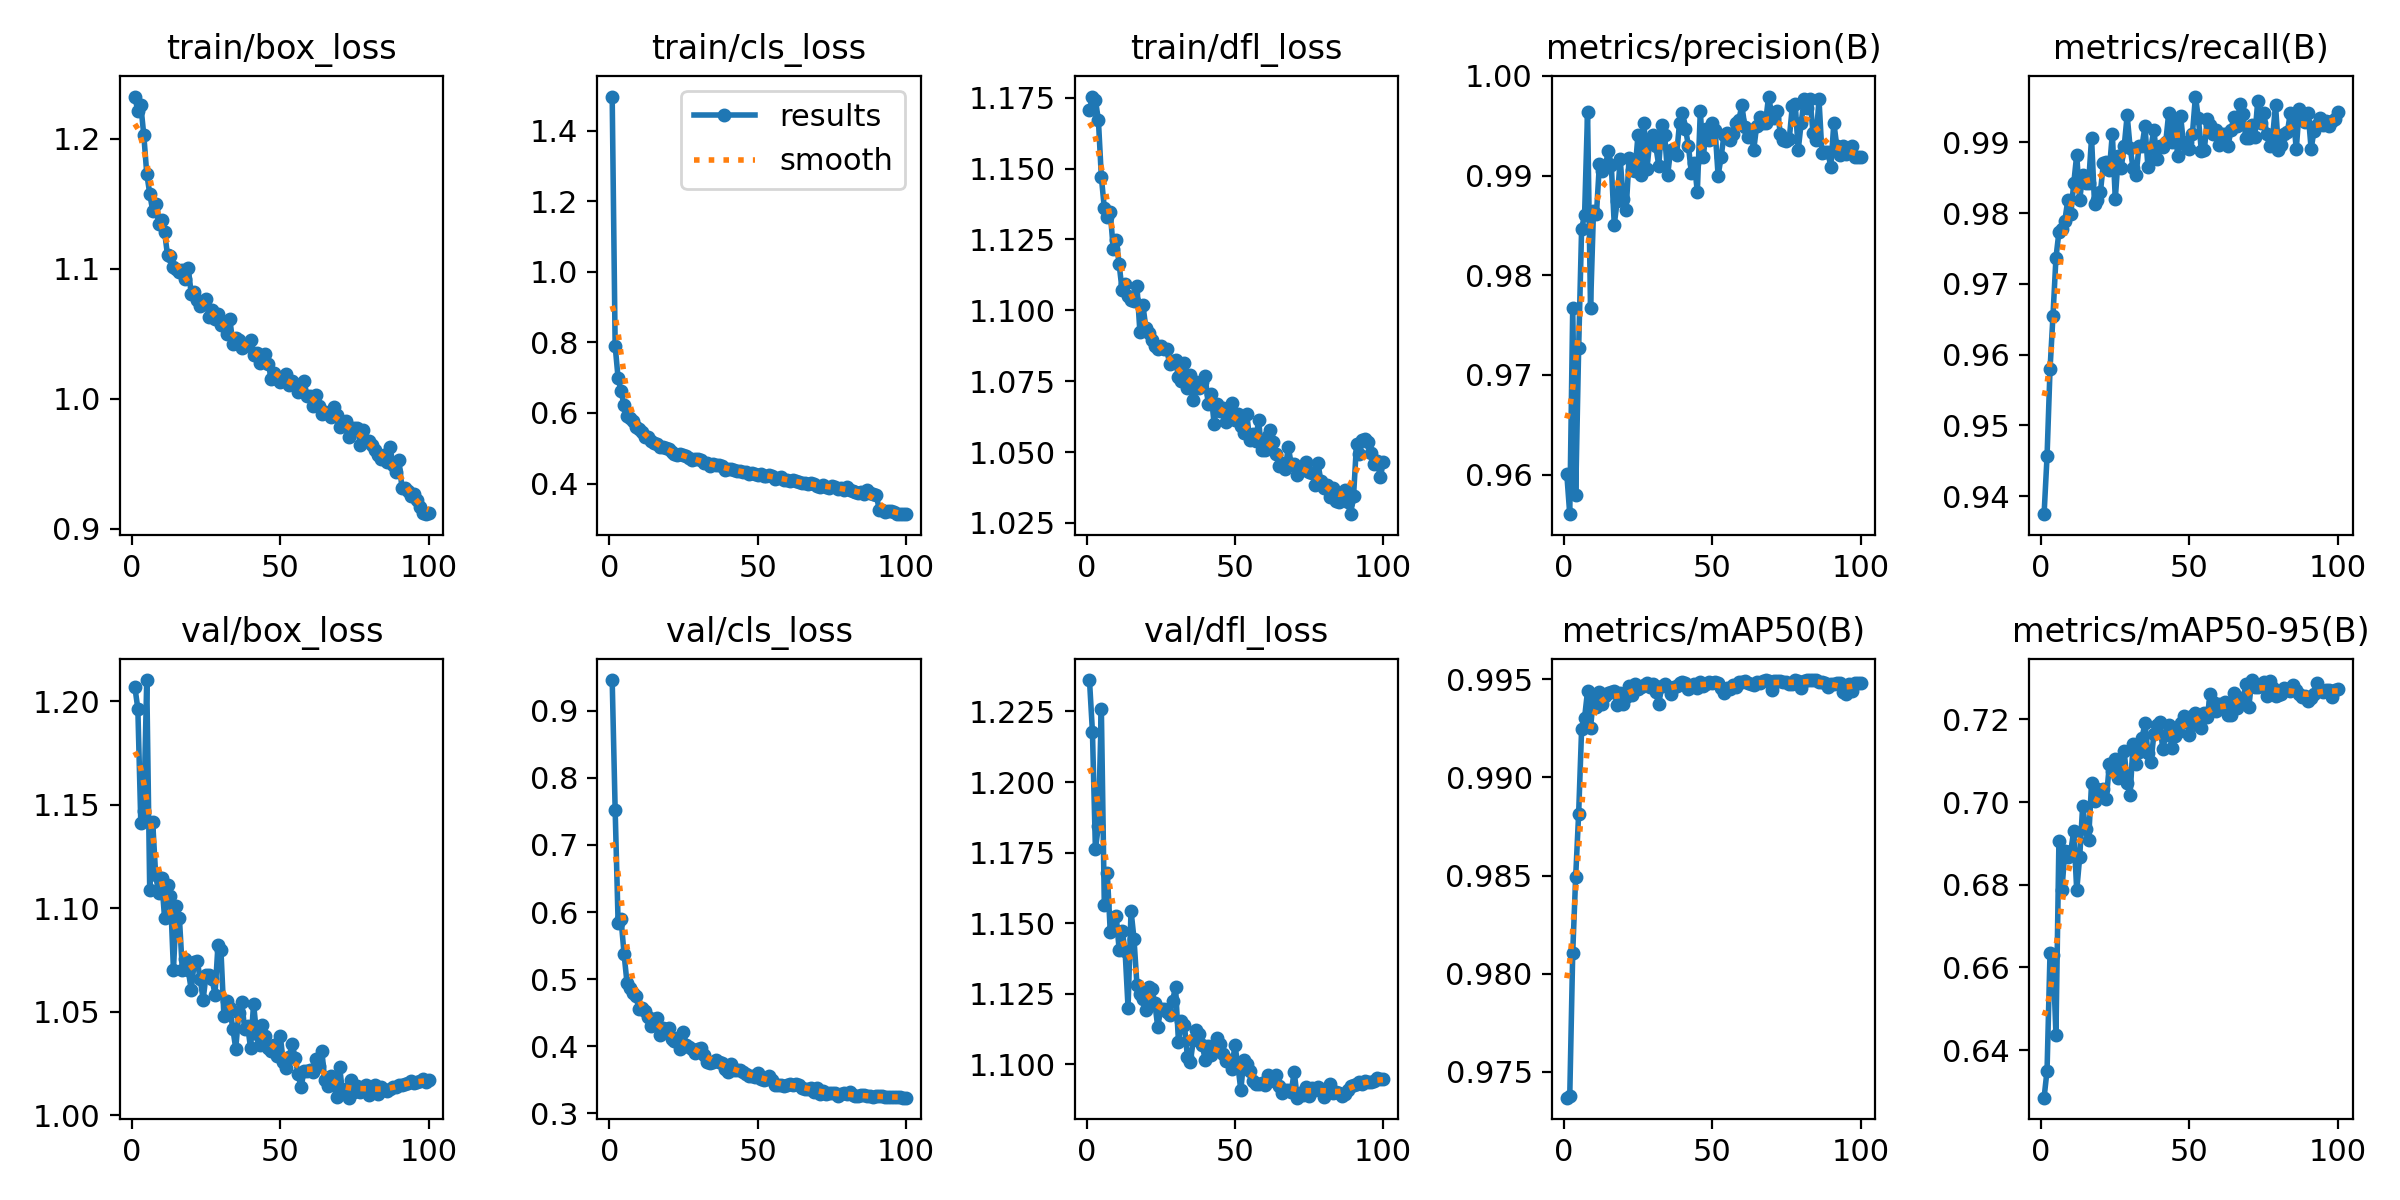
\includegraphics[height=0.55\textheight]{results.png}
    \end{figure}
    \begin{itemize}
        \item \textbf{Độ chính xác (mAP50):} Đạt \textbf{99.1\%}, mô hình nhận diện chính xác vùng biển số trong mọi điều kiện.
    \end{itemize}
\end{frame}

\begin{frame}{4. So sánh tiền xử lý cho PaddleOCR}
    \begin{itemize}
        \item Đánh giá trên bộ dữ liệu 6,432 biển số Việt Nam.
    \end{itemize}
    \begin{figure}
        \centering
        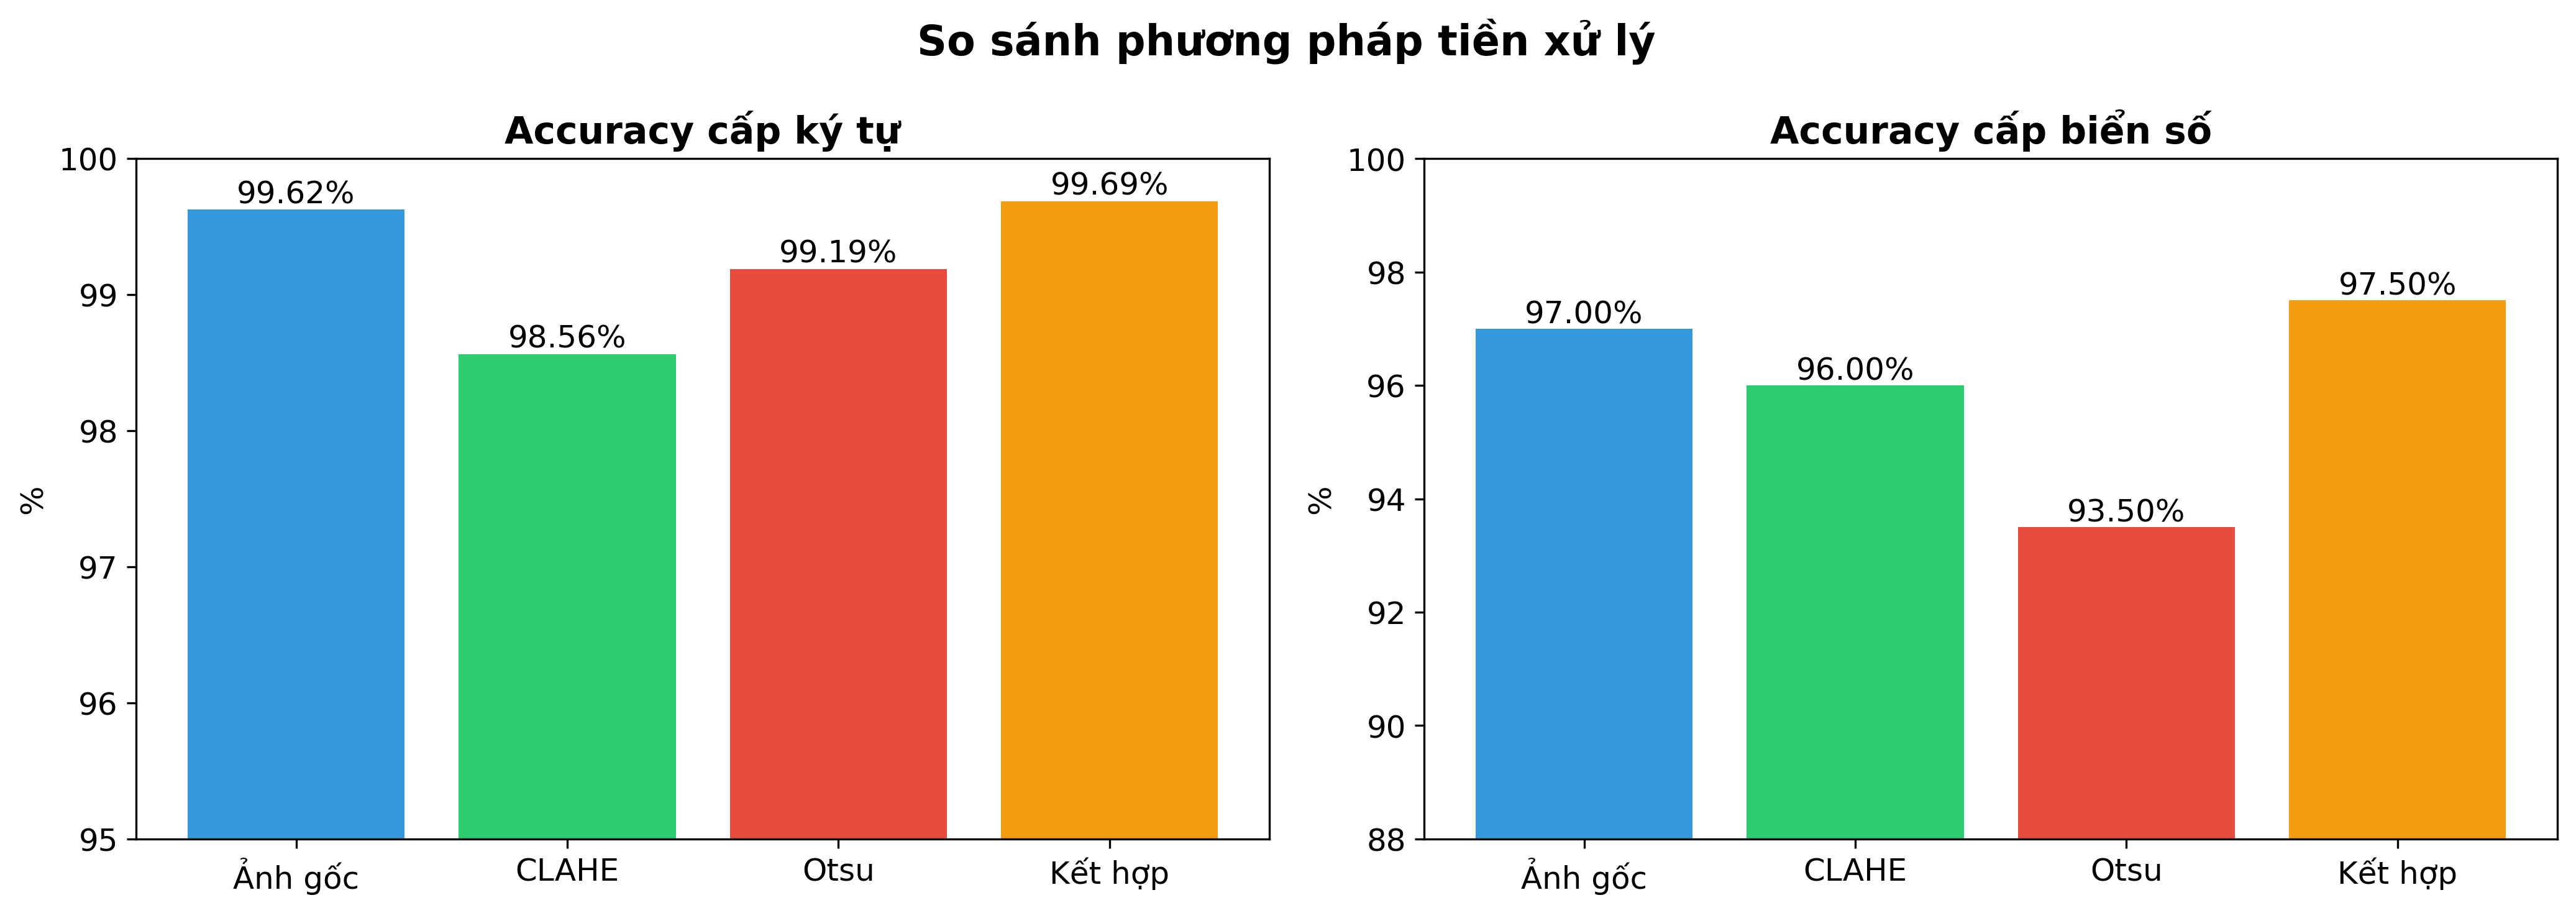
\includegraphics[height=0.6\textheight]{so_sanh_tien_xu_ly.png}
    \end{figure}
\end{frame}

\begin{frame}{4. Đánh giá độ chính xác OCR (Ma trận nhầm lẫn)}
    \begin{figure}
        \centering
        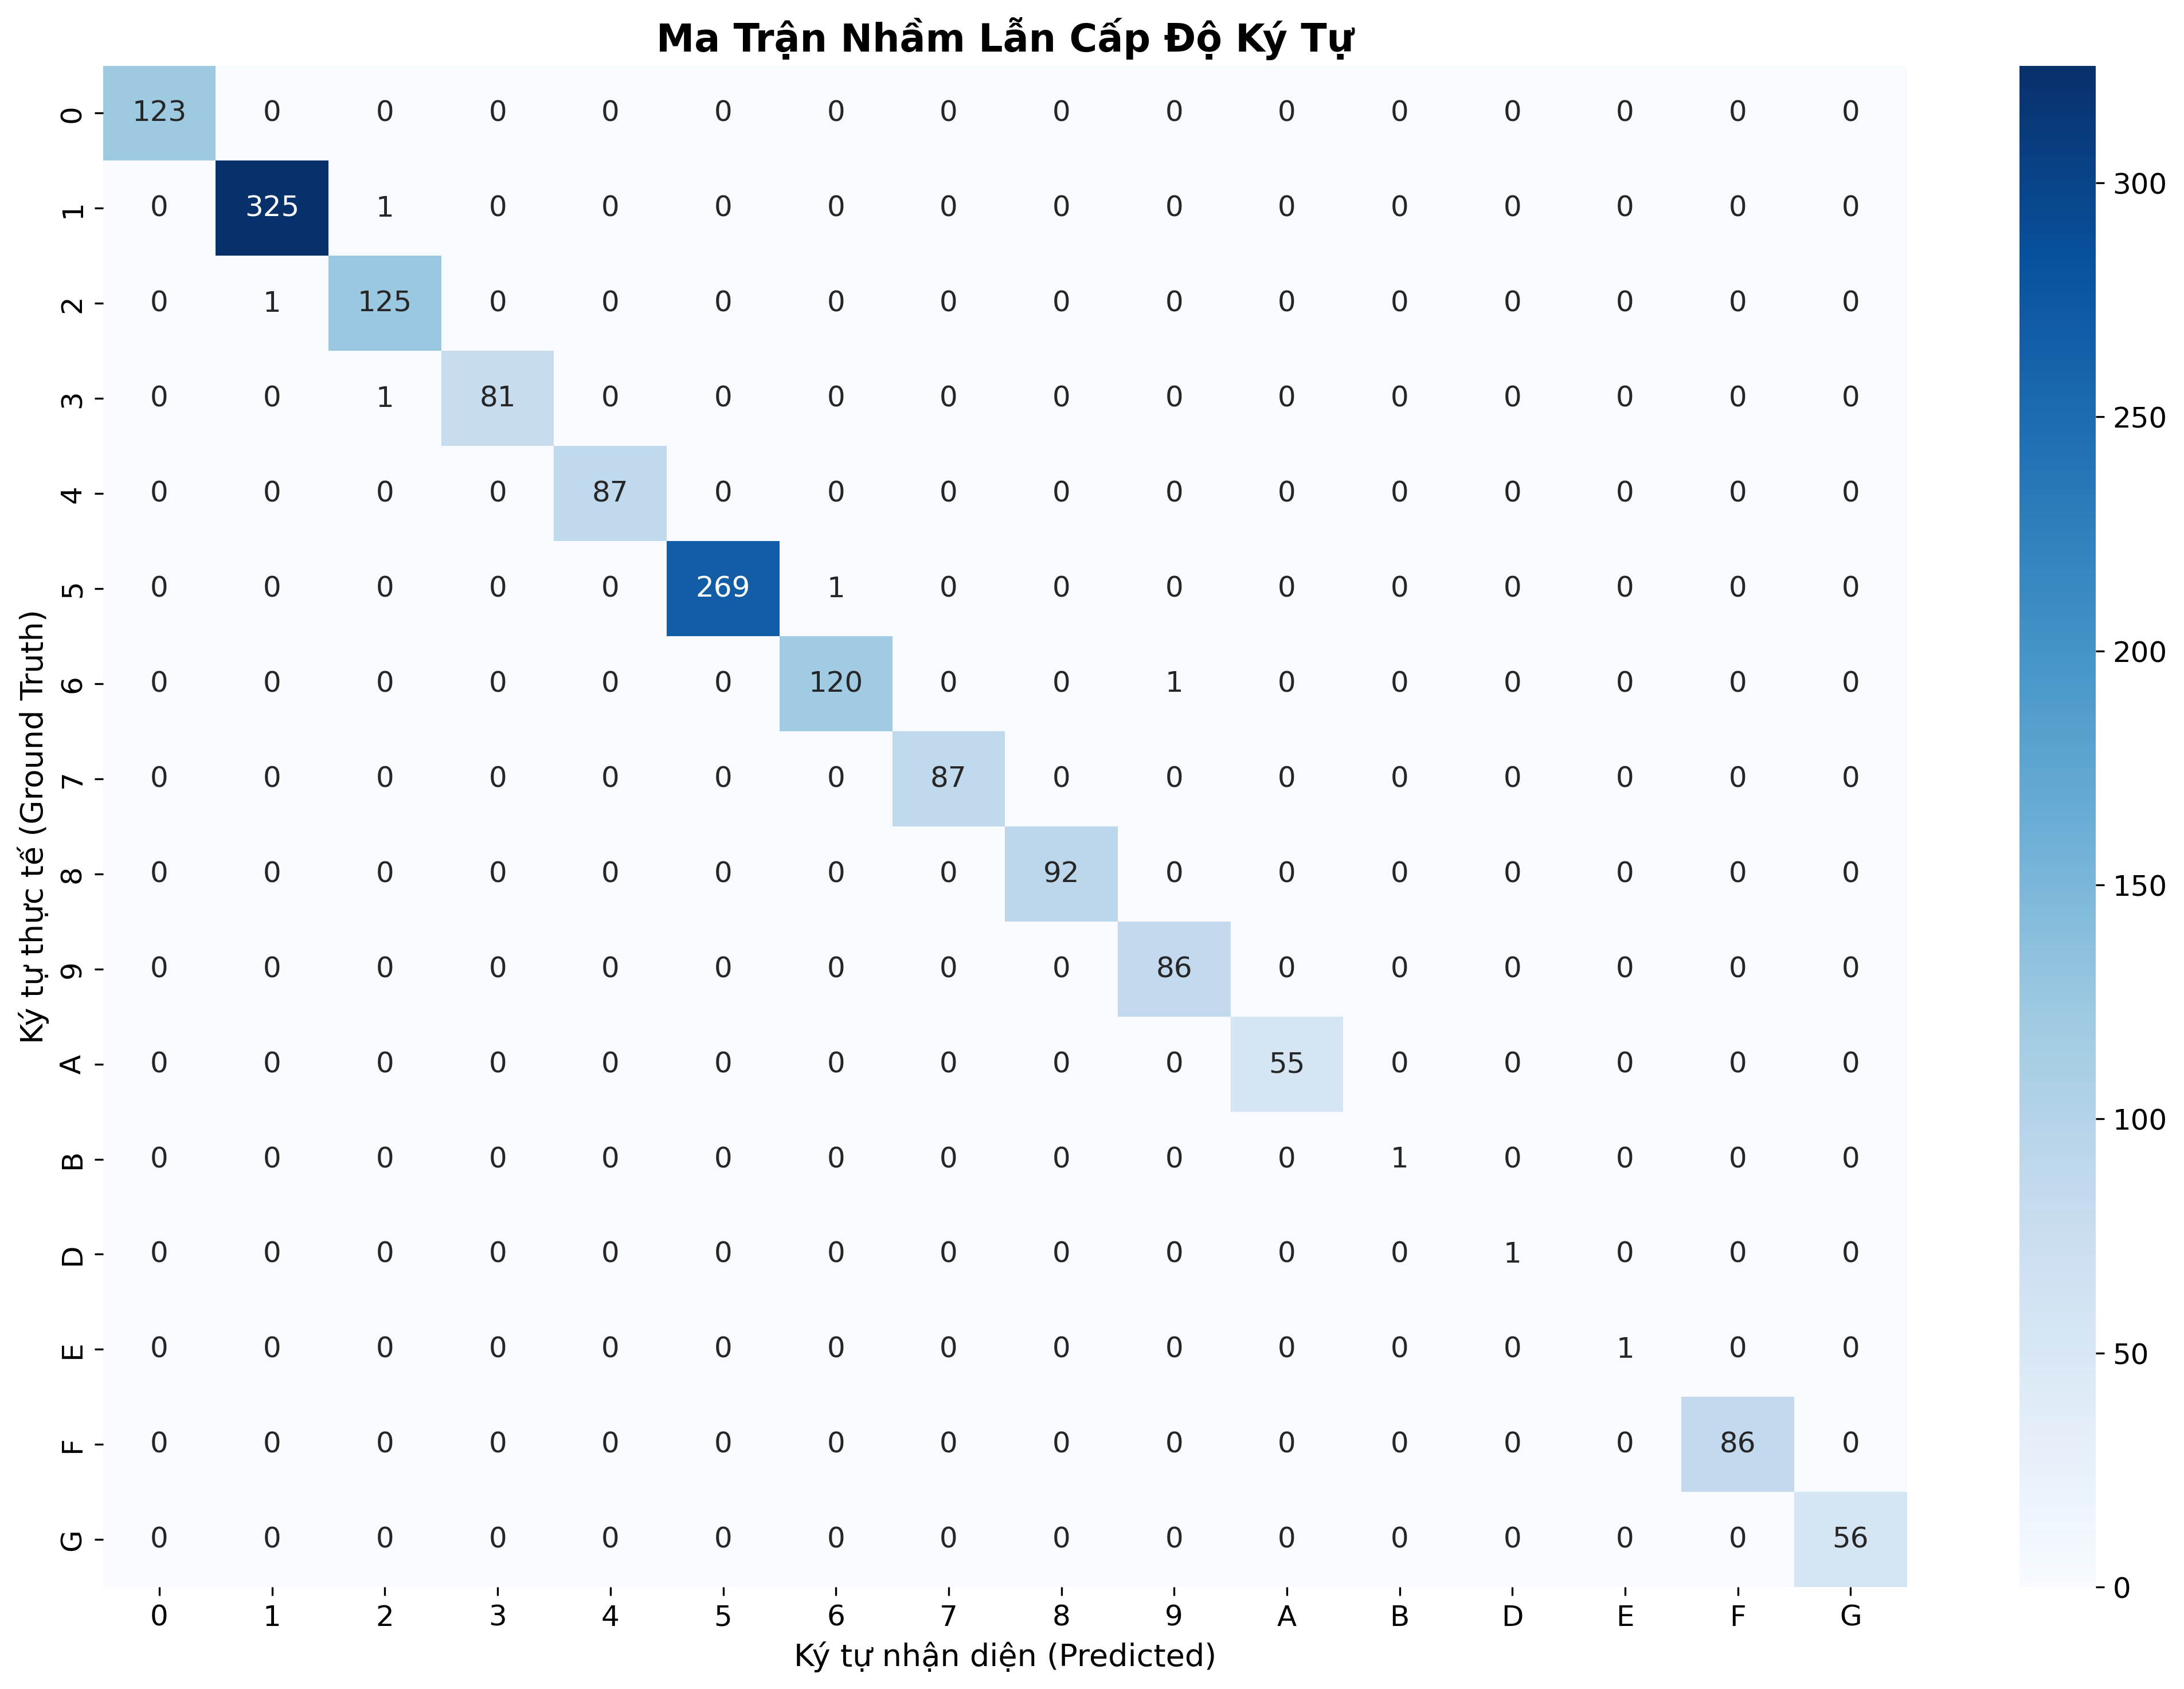
\includegraphics[height=0.75\textheight]{confusion_matrix_kytu.png}
    \end{figure}
\end{frame}

\begin{frame}{4. Giao diện phần mềm quản lý}
    \begin{itemize}
        \item Giao diện được thiết kế bằng \textbf{CustomTkinter} hiện đại.
        \item Hỗ trợ luồng camera trực tiếp, hiển thị kết quả AI và ghi CSDL ngay lập tức.
    \end{itemize}
\end{frame}

% --- Phần 5: Kết luận ---
\section{Kết luận}
\begin{frame}{5. Kết luận và Hướng phát triển}
    \textbf{Kết quả đạt được:}
    \begin{itemize}
        \item Xây dựng thành công hệ thống bãi đỗ xe tự động từ phần cứng đến phần mềm.
        \item Tối ưu pipeline YOLOv8 + PaddleOCR đạt độ chính xác cao >96\%.
        \item Hệ thống hoạt động trơn tru với cơ chế đa luồng thời gian thực.
    \end{itemize}
    \vspace{0.5cm}
    \textbf{Hướng phát triển tương lai:}
    \begin{itemize}
        \item Nhận diện thêm đặc điểm xe (màu sắc, loại xe).
        \item Ứng dụng thuật toán ghép luồng nhiều camera cho các bãi đỗ lớn.
        \item Triển khai ứng dụng Web/Mobile để khách hàng tự theo dõi xe.
    \end{itemize}
\end{frame}

\begin{frame}
    \centering
    \Huge \textbf{XIN CẢM ƠN QUÝ THẦY CÔ VÀ CÁC BẠN ĐÃ LẮNG NGHE!}
\end{frame}

\end{document}
